%\addchap{Anhang E}
%\setcounter{chapter}{5}
%\setcounter{section}{0}
%\setcounter{table}{0}
%\setcounter{figure}{0}
%
%\section{Wichtige \LaTeX -Befehle}
%
%\begin{tabbing}
%\hspace*{0cm} \= \hspace{0.28\linewidth} \= \+\kill
%\textbackslash \textit{label}\{\}	\> Definition eines Labels, auf welches referenziert werden kann\\ 
%	\> z.B.: \textbackslash \textit{label}\{fig:MyImage\}\\ 
%\textbackslash \textit{ref}\{\}	\> Setzen einer Referenz zu einem Label\\
%\textbackslash \textit{pageref}\{\}	\> Gibt die Seitenzahl zu einer Referenz zurück\\
%	\> z.B.: Tabelle\~{}\textbackslash \textit{ref}\{tab:messdaten\} fasst die Messergebnisse zusammen.\\ 
%\textbackslash \textit{cite}\{\}	\> Literaturreferenz einfügen\\
%\textbackslash \textit{cite}[S. x]\{\}	\> Literaturreferenz mit Angabe einer Seitenzahl \glqq x\grqq~einfügen\\
%
%\textbackslash \textit{footnote}\{\}	\> Fußnote einfügen\\ 
%\~{}	\> Einfügen eines geschützten Leerzeichens\\ 
%\textdollar \textit{Formel} \textdollar	\> Eingabe einer Formel im Text\\
%\textbackslash \textit{nomenclature}\{a.\}\{ab\}	\> Aufnahme der Abkürzung \glqq a.\grqq~für \glqq ab\grqq~in das Abkürzungsverzeichnis.\\
%\textbackslash \textit{index}\{Obst!Birne\} \> Aufnahme des Begriffs \glqq Birne\grqq~in den Index unter \glqq Obst\grqq. \index{Obst!Birne} \\
%\textbackslash \textit{clearpage}	\> Ausgabe aller Gleitobjekte und Umbruch auf neue Seite\\ 
%\end{tabbing}
%
%\clearpage
%
%\section{Vorlagen für \LaTeX Umgebungen}
%
%\subsection{Listen und Aufzählungen}
%
%Es gibt folgende Listentypen. Die wichtigsten:
%
%\begin{itemize}
%	\item Einfache Liste mit \textit{itemize}-Umgebung
%	\item ...
%\end{itemize}
%
%\begin{enumerate}
%	\item Nummerierte Liste mit \textit{enumerate}-Umgebung
%	\item ...
%\end{enumerate}
%
%\begin{enumerate}[label=\alph*.]
%	\item wobei man bei der \textit{enumerate}-Umgebung leicht die Art der Nummerierung ändern kann,
%	\item ...
%\end{enumerate}
%
%und durch verschachtelte Umgebungen verschiedene Aufzählungsebenen darstellen kann:
%
%\begin{enumerate}[label=\alph*)]
%	\item Erster Aufzählungspunkt der ersten Ebene
%	\item ...
%	\begin{itemize}
%		\item Erster Punkt der zweiten Ebene
%		\item Zweiter Punkt der zweiten Ebene
%	\end{itemize}
%	\item Das sollte an Beispielen zunächst einmal genügen.
%\end{enumerate}
%
%\clearpage
%
%\subsection{Bilder und Grafiken}
%
%Bilder können als PDF-, JPG-, und PNG-Bilder in \LaTeX eingebunden werden. Damit eine Grafik in hoher Qualität dargestellt wird, sollte das Dateiformat der Grafik vektorbasiert sein, d.h. als PDF-Datei vorliegen. Viele Zeichenprogramme unterstützen einen PDF-Export (z.B. GIMP, Adobe Illustrator, etc.). Für Grafiken aus PowerPoint sei folgende Vorgehensweise beim Export empfohlen:
%
%\begin{enumerate}
%	\item Die gewünschte Grafik in PowerPoint zeichnen.
%	\item Gewünschten Bildbereich markieren, rechte Maustaste klicken und \glqq Als Grafik speichern ...\grqq~wählen.
%	\item Grafik im Format EMF abspeichern. Das EMF-Format ist vektorbasiert.\footnote{Mit dem Mac kann in PowerPoint die Grafik direkt im PDF-Format exportiert werden. Die weiteren Schritte entfallen daher.}
%	\item Mit dem Programm XnView die Grafik im EMF-Format in PDF wandeln und abspeichern.
%	\item Die so erzeugte PDF-Datei enthält eine vektorbasierte Grafik und kann in \LaTeX~ eingebunden werden.
%\end{enumerate}
%
%Abbildung~\ref{fig:MyImage} zeigt ein Beispielbild einer Grafik, welche aus PowerPoint exportiert wurde.
%
%\begin{figure}[hbt]
%	\centering
%	
\includegraphics[width=0.3\linewidth]{images/MyImage}
%	\caption[Beispiel für die Einbindung eines Bildes.]{Beispiel für die Einbindung eines Bildes (PDF-, JPG-, und PNG-Bilder können eingebunden werden).}
%	\label{fig:MyImage}
%\end{figure}
%
%Der Quellcode des Beispielbildes aus Abbildung~\ref{fig:MyImage} ist in Listing~\ref{lst:fig} zu sehen.
%
%\clearpage
%
%\begin{lstlisting}[caption=Quellcode der Abbildung~\ref{fig:MyImage}.,label=lst:fig]
%\begin{figure}[hbt]				% here, bottom, top
%\centering						% Zentrierung
%
\includegraphics[width=0.6\linewidth]{images/MyImage}		
%\caption[Beispiel für die Einbindung eines Bildes.]{Beispiel für die Einbindung eines Bildes (PDF-, JPG-, und PNG-Bilder können eingebunden werden).}
%\label{fig:MyImage}
%\end{figure}
%\end{lstlisting}
%
%Grafiken können auch mithilfe des Packages Tikz gezeichnet, bzw. programmiert werden. Grafiken mit Tikz werden mit dem \textit{input}-Befehl in die \textit{figure}-Umgebung geladen, wie nachfolgendes Beispiel in Abbildung~\ref{fig:tikz_house} zeigt:
%
%\begin{figure}[hbt]
%	\centering
%	 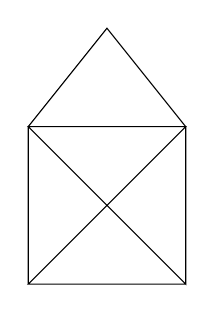
\begin{tikzpicture}
\draw (0,0) -- (0,2) -- (1,3.25) -- (2,2) -- (2,0) -- (0,2) -- (2,2) -- (0,0) -- (2,0);
\end{tikzpicture}
    
%	\caption[Mit Tikz programmierte Grafik.]{Mit Tikz programmierte Grafik.}
%	\label{fig:tikz_house}
%\end{figure}
%
%Ein etwas umfangreicheres Beispiel zur Digitaltechnik ist in Abbildung~\ref{fig:tikz_digital} dargestellt:
%
%\begin{figure}[hbt]
%	\centering
%	\usetikzlibrary{circuits.logic.US,circuits.logic.IEC}
      \begin{tikzpicture}[circuit logic US]
      \matrix[column sep=7mm]
      {
      \node (i0) {0}; & & \\
      & \node [and gate] (a1) {}; & \\
      \node (i1) {0}; & & \node [or gate] (o) {};\\
      & \node [nand gate] (a2) {}; & \\
      \node (i2) {1}; & & \\
      };
      \draw (i0.east) -- ++(right:3mm) |- (a1.input 1);
      \draw (i1.east) -- ++(right:3mm) |- (a1.input 2);
      \draw (i1.east) -- ++(right:3mm) |- (a2.input 1);
      \draw (i2.east) -- ++(right:3mm) |- (a2.input 2);
      \draw (a1.output) -- ++(right:3mm) |- (o.input 1);
      \draw (a2.output) -- ++(right:3mm) |- (o.input 2);
      \draw (o.output) -- ++(right:3mm) node [right] {$y$ \quad Hier könnte Ihre Formel $y=(0 \land 0) \lor \overline{( 0 \land 1)}$ stehen};
 \end{tikzpicture}

%	\caption[Mit Tikz programmierte Grafik, welche bereits vorgefertigte Bibliotheken für Symbole aus der Digitaltechnik nutzt.]{Mit Tikz programmierte Grafik, welche bereits vorgefertigte Bibliotheken für Symbole aus der Digitaltechnik nutzt.}
%	\label{fig:tikz_digital}
%\end{figure}
%
%\clearpage
%
%In der Tikz-Umgebung können auch Diagramme mit dem \textit{pgfplot}-Befehlssatz erzeugt werden. In Abbildung \ref{fig:pgfplot} sehen Sie ein Beispiel.
%
%\begin{figure}[hbt]
%	\centering
%	\begin{tikzpicture}
		\begin{axis}[scale=1.3,legend entries={Messwerte mit Fehlerbalken,
			$\pgfmathprintnumber{\pgfplotstableregressiona} \cdot x  
			\pgfmathprintnumber[print sign]{\pgfplotstableregressionb}$}, legend style={draw=none},legend style={at={(0.01,0.98)},anchor=north west},xlabel=Stromstärke $I \; \mathrm{ \lbrack mA \rbrack}$,ylabel=Spannung $U \; \mathrm{ \lbrack V \rbrack}$]
		\addlegendimage{mark=*,blue}
		\addlegendimage{no markers,red}
\addplot+[error bars/.cd, y dir=both,y explicit]
table[x=x,y=y,y error=errory] 
{pgfplot/messdaten_mitfehler.dat};
\addplot table[mark=none,y={create col/linear regression={y=y}}]
{pgfplot/messdaten_mitfehler.dat};
	\end{axis}
\end{tikzpicture}
%	\caption[Diagramm, erstellt mit dem \textit{pgfplot}-Befehlssatz.]{Ein Diagramm, erstellt in der \textit{tikzpicture}-Umgebung mit dem \textit{pgfplot}-Befehlssatz. Das Diagramm stellt Messdaten, deren Fehlerbalken und eine Regressionskurve dar. Die Messdaten werden von einer separaten Datei eingelesen und die Regressionskurve wurde mit \textit{pgfplot} berechnet und erstellt.}
%	\label{fig:pgfplot}
%\end{figure}
%
%\clearpage
%
%Auch hierzu der Quellcode in Listing~\ref{lst:pgfplot}.
%
%\begin{lstlisting}[caption=Quellcode der Abbildung~\ref{fig:pgfplot}.,label=lst:pgfplot]
%\begin{figure}[hbt]
%\centering
%\begin{tikzpicture}
		\begin{axis}[scale=1.3,legend entries={Messwerte mit Fehlerbalken,
			$\pgfmathprintnumber{\pgfplotstableregressiona} \cdot x  
			\pgfmathprintnumber[print sign]{\pgfplotstableregressionb}$}, legend style={draw=none},legend style={at={(0.01,0.98)},anchor=north west},xlabel=Stromstärke $I \; \mathrm{ \lbrack mA \rbrack}$,ylabel=Spannung $U \; \mathrm{ \lbrack V \rbrack}$]
		\addlegendimage{mark=*,blue}
		\addlegendimage{no markers,red}
\addplot+[error bars/.cd, y dir=both,y explicit]
table[x=x,y=y,y error=errory] 
{pgfplot/messdaten_mitfehler.dat};
\addplot table[mark=none,y={create col/linear regression={y=y}}]
{pgfplot/messdaten_mitfehler.dat};
	\end{axis}
\end{tikzpicture}
%\caption[Diagramm, erstellt mit dem \textit{pgfplot}-Befehlssatz.]{Ein Diagramm, erstellt in der \textit{tikzpicture}-Umgebung mit dem \textit{pgfplot}-Befehlssatz. Das Diagramm stellt Messdaten, deren Fehlerbalken und eine Regressionskurve dar. Die Messdaten werden von einer separaten Datei eingelesen und die Regressionskurve wurde mit \textit{pgfplot} berechnet und erstellt.}
%\label{fig:pgfplot}
%\end{figure}
%\end{lstlisting}
%
%In Listing~\ref{lst:tikz} ist der Quellcode der Datei \textit{mess\_fehlerbalken.tex} dargestellt.
%
%\begin{lstlisting}[caption=Quellcode der Datei \textit{mess\_fehlerbalken.tex}.,label=lst:tikz]
%\begin{tikzpicture}
%\begin{axis}[scale=1.3,legend entries={Messwerte mit Fehlerbalken,
%$\pgfmathprintnumber{\pgfplotstableregressiona} \cdot x  
%\pgfmathprintnumber[print sign]{\pgfplotstableregressionb}$}, legend style={draw=none},legend style={at={(0.01,0.98)},anchor=north west},xlabel=Stromstärke $I \; \mathrm{ \lbrack mA \rbrack}$,ylabel=Spannung $U \; \mathrm{ \lbrack V \rbrack}$]
%\addlegendimage{mark=*,blue}
%\addlegendimage{no markers,red}
%\addplot+[error bars/.cd, y dir=both,y explicit]
%table[x=x,y=y,y error=errory] 
%{pgfplot/messdaten_mitfehler.dat};
%\addplot table[mark=none,y={create col/linear regression={y=y}}]
%{pgfplot/messdaten_mitfehler.dat};
%\end{axis}
%\end{tikzpicture}
%\end{lstlisting}
%
%\clearpage
%
%In Abbildung~\ref{fig:pgfplot2y} wird ein weiters Beispiel für ein Diagramm gezeigt. Oftmals wird eine zweite y-Achse verwendet, um verschiedene Skalen darstellen zu können.
%
%\begin{figure}[hbt]
%	\centering
%	\begin{tikzpicture}
%
\begin{axis}[
scale=1.3,
ytick pos=left,
xlabel=Zeit $t \; \mathrm{ \lbrack ns \rbrack}$,
ylabel=Spannung $U \; \mathrm{ \lbrack V \rbrack}$
]
\addplot[mark=*,only marks] table[x=x,y=y1] {pgfplot/messdaten_zweiyachsen.dat};
\end{axis}
%
\begin{axis}[
scale = 1.3,
legend style={draw=none},
legend style={at={(0.75,0.6)},
anchor=north west},
axis y line*=right,
axis x line=none,
%ymin=0,
%ymax=100,
ylabel=Strom $I \; \mathrm{ \lbrack mA \rbrack}$
]
\addlegendimage{mark=*,only marks}
\addlegendentry{Spannung}
\addplot[mark=x,only marks,blue] table[x=x,y=y2] {pgfplot/messdaten_zweiyachsen.dat};
\addlegendentry{Strom}
\end{axis}
\end{tikzpicture}
%	\caption[Diagramm mit zwei unterschiedlichen y-Achsen.]{Diagramm mit zwei unterschiedlichen y-Achsen.}
%	\label{fig:pgfplot2y}
%\end{figure}
%
%\clearpage
%
%\subsection{Tabellen}
%
%\begin{table}[hbt]	
%	\centering
%	\renewcommand{\arraystretch}{1.5}	% Skaliert die Zeilenhöhe der Tabelle
%	\captionabove[Liste der verwendeten Messgeräte]{Liste der verwendeten Messgeräte. Die Genauigkeitsangaben beziehen sich auf die Standardabweichung $1\cdot \sigma$.}
%	\label{tab:bsp}
%	\begin{tabular}{ccccc}
%		\textbf{Messgerät} & \textbf{Hersteller} & \textbf{Typ} & \textbf{Verwendung} & \textbf{Genauigkeit}\\ 
%		\hline 
%		\hline 
%		\parbox[t]{0.2\linewidth}{\centering Spannungs-\\versorgung} & Voltmaker & HV2000 & \parbox[t]{0.2\linewidth}{\centering Spannungs-\\versorgung der\\Platine} & $\Delta U = \pm 5 $~mV \\ % Der parbox-Befehl ist erforderlich, damit ein Zeilenumbruch erzeugt werden kann. c-Spalten (zentriert) erlauben nicht automatisch einen Zeilenumpruch. Linksbündig gesetzte p-Spalten erlauben automatisch den Zeilenumbruch.
%		Strommessgerät & Currentcount & Hotamp 16 & \parbox[t]{0.2\linewidth}{ \centering Strommessung\\am Versorgungspin\\des µC} & $\Delta I = \pm 0.1$~A \\ 
%		\hline 
%	\end{tabular} 
%\end{table}
%
%Der Quellcode der Beispieltabelle~\ref{tab:bsp} ist in Listing~\ref{lst:tab} zu sehen.
%
%\begin{lstlisting}[caption=Quellcode der Tabelle~\ref{tab:bsp}.,label=lst:tab]
%\begin{table}[hbt]	
%\centering
%\renewcommand{\arraystretch}{1.5}	% Skaliert die Zeilenhöhe der Tabelle
%\captionabove[Liste der verwendeten Messgeräte]{Liste der verwendeten Messgeräte. Die Genauigkeitsangaben beziehen sich auf die Standardabweichung $1\cdot \sigma$.}
%\label{tab:bsp}
%\begin{tabular}{ccccc}
%\textbf{Messgerät} & \textbf{Hersteller} & \textbf{Typ} & \textbf{Verwendung} & \textbf{Genauigkeit}\\ 
%\hline 
%\hline 
%\parbox[t]{0.2\linewidth}{\centering Spannungs-\\versorgung} & Voltmaker & HV2000 & \parbox[t]{0.2\linewidth}{\centering Spannungs-\\versorgung der\\Platine} & $\Delta U = \pm 5 $~mV \\ % Der parbox-Befehl ist erforderlich, damit ein Zeilenumbruch erzeugt werden kann. c-Spalten (zentriert) erlauben nicht automatisch einen Zeilenumpruch. Linksbündig gesetzte p-Spalten erlauben automatisch den Zeilenumbruch.
%Strommessgerät & Currentcount & Hotamp 16 & \parbox[t]{0.2\linewidth}{ \centering Strommessung\\ am Versorgungspin\\ des \textmu C} & $\Delta I = \pm 0.1$~A \\ 
%\hline 
%\end{tabular} 
%\end{table}
%\end{lstlisting}
%
%\clearpage
%
%\subsection{Formeln}
%
%Formeln lassen sich in \LaTeX~ganz einfach schreiben. Es gibt unterschiedliche Umgebungen zum Schreiben von Formeln. Z.B. direkt im Text $v=s/t$ oder abgesetzt
%
%\[F=m \cdot a\]
%
%oder auch, wie in wissenschaftlichen Dokumenten üblich, nummeriert
%
%\begin{equation}
%P=\frac{U^2}{R} \quad .
%\label{eqn:leistung}
%\end{equation}
%
%Mit einem Label in Formel~\ref{eqn:leistung} lassen sich natürlich auch Formeln im Text referenzieren. \LaTeX~verwendet im Formelmodus einen eigenen Schriftsatz, welcher entsprechend der gängigen Konventionen kursive Zeichen verwendet. Sollen im Formelmodus Einheiten in normaler Schriftart eingefügt werden, dann kann dies über den Befehl \textbackslash \textit{mathrm}\{\} erwirkt werden, wie im Quellcode von Formel~\ref{eqn:leistungMitEinh} zu sehen ist.
%
%\begin{equation}
%P=\frac{U^2}{R} = \frac{\left( 100~\mathrm{V}\right)^2}{100~\Omega} = 100~\mathrm{W}\quad .
%\label{eqn:leistungMitEinh}
%\end{equation}
%
%Zum direkten Vergleich sind die Einheiten in Formel~\ref{eqn:leistungMitEinhfalsch} falsch dargestellt:
%
%\begin{equation}
%P=\frac{U^2}{R} = \frac{\left( 100~V\right)^2}{100\,\varOmega} = 100\,W
%\label{eqn:leistungMitEinhfalsch}
%\end{equation}
%
%Zur einfachen Eingabe von Einheiten kann auch das Package \textbackslash \textit{siunitx} verwendet werden:
%
%\begin{equation}
%	P=\SI{100}{\watt}=\SI{100}{\joule\per\second}
%\end{equation}
%
%Das sind nur ein paar wenige Beispiele und es gibt sehr viele Packages, um Besonderheiten in Formeln realisieren zu können, z.B. mehrzeilige Formeln mit vertikaler Ausrichtung. Nennen Sie Formeln nur, wenn diese zum besseren Verständnis auch wirklich nützlich sind.
%
%Folgende Befehle sind innerhalb von Formel-Umgebungen nützlich:
%\begin{tabbing}
%	\hspace*{0cm} \= \hspace{0.35\linewidth} \= \+\kill
%	\textbackslash \textit{text}\{\}	\> Damit kann in Formel-Umgebung Text geschrieben werden.\\ 
%	\textbackslash, \textbackslash: \textbackslash; oder \textbackslash quad und \textbackslash qquad \> Zusätzlichen Abstand zwischen Symbolen einfügen.\\
%	\textbackslash \textit{notag} \> Nummerierung einer bestimmten Formel ausschalten.
%\end{tabbing}
%
%Abschließend nochmals ein kleines Beispiel:
%
%\begin{eqnarray}
%\sum\limits_{n=1}^\infty f\left(x_n\right)\cdot \Delta x=  \lim\limits_{\Delta x \rightarrow 0} \frac{f\left(x_0+\Delta x\right)-f\left(x_0\right)}{\Delta x} = \frac{\diff f}{\diff x} = \dot{f}(x)
%\end{eqnarray}